\chapter{Client-to-LAN VPN}

\section{Virtual Private Networks (VPN)}
Ein "`Virtual Private Network"' (VPN) bezeichnet ein privates Netzwerk, welches innerhalb einer öffentlichen Netzwerkinfrastruktur, zumeist dem Internet, aufgebaut wird. Der Zugang ist so beschränkt, dass nur Mitglieder einer vordefinierten Gruppe an diesem privaten Netzwerk teilnehmen können. Zumeist werden dabei geographisch verteilte (Sub-) Netzwerke, die einer gemeinsamen administrativen Domäne (z.B. einer Firma oder einer Behörde) angehören, mittels der öffentlichen Infrastruktur aneinander gekoppelt. Der Verkehr, der dabei über die öffentliche Infrastruktur geleitet wird, wird dabei in der Regel verschlüsselt \cite{Ferguson1998}. Im vorliegenden Fall ist die öffentliche Infrastruktur das simulierte Internet, welches außerhalb der Netzwerke der beiden Firmen liegt. Es werden allerdings keine Netzwerke miteinander verknüpft, sondern lediglich einzelne Clients (um genau zu sein ein einziger Client) mit einem Netzwerk, dem internen LAN der Firma A, verbunden. Die Zugangsbeschränkung ist Zertifikatsbasiert \cite{Neuschwander2014}.

\subsection{OpenVPN}
OpenVPN ist eine freie Software zur Herstellung von VPN. Es ist für alle gängigen Betriebssysteme erhältlich und nutzt zur Verschlüsselung, Authentisierung und Zertifizierung die OpenSSL-Bibliothek \cite{OpenVPNeu}. OpenVPN gewährt ein hohes Maß an Wahlfreiheit bezüglich des verwendeten Protokolls (TCP/UDP), der Authentisierungsmethode (Pre-Shared-Key, Benutzername/Passwort, Zertifikatsbasiert), Nutzung eines VPN-Tunnels oder einer ethernet-bridge, sowie zwischen symmetrischer und Public-Key Verschlüsselung. OpenVPN ermöglicht es dabei, auch Verbindungen mit Netzwerken herzustellen, deren Schnittstelle zum Öffentlichen Netzwerk dynamisch sind (z.B. bei dynamischen IP-Adressen) \cite{wiOpenVPN}. Entwickelt und betreut wird es von OpenVPN Technologies, Inc..

\section{Aufgabenstellung}

Mitarbeiter von Firma A, sollen die Möglichkeit haben von überall arbeiten zu können, und von dort auch Zugriff auf das interne Firmen Netzwerk zu erhalten.
Vorrausgesetzt wird hierbei selbstverständlich der Zugang zum Internet.

Realisiert werden soll dies mittels einer Client-to-LAN VPN-Verbindung die technisch mittels der freien Software \emph{OpenVPN} implementiert werden soll.

\section{Implementierung}

Um eine Verbindung zwischen einem externen Mitarbeiter bzw. dem externen Gerät und dem internen Netzwerk von Firma A herstellen zu können, muss einerseits ein \textbf{Server} den VPN Dienst anbieten und andererseits muss der \textbf{Client} des Mitarbeiters so konfiguriert sein, dass er sich mit diesem Dienst verbinden kann.
Als Server dient die innere Firewall fw2.firma-a.f223, denn nur auf dieser besteht die Möglichkeit den VPN-Server so einzurichten, dass die sich verbindenden Clients Zugriff auf das Intranet erhalten.
Beim zu konfigurierenden Client handelt es sich um den externen Laptop lap01.internet.f223 \cite{Neuschwander2014}.

Im Folgenden wird die Installation und Konfiguration der OpenVPN Software auf Client und Server erläutert.


\subsection{Server}\label{vpn:server}

Auf der internen Firewall von Firma a müssen zunänchst die benötigten Software Packete installiert werden. Hierbei handelt es sich um das Packet \texttt{openvpn}, welches die OpenVPN Software enthält. Zusätzlich wird das Packet \texttt{bridge-utils} benötigt.
Es wird zur Konfiguration der Bridge zwischen des von OpenVPN bereitgestellten Neztwerkinterfaces \texttt{tap0}, und der normalen Netzwerkschnittstelle \texttt{eth0}, die mit dem Intranet verbunden ist, benötigt.

Die Installation der Packete erfolgt mittels der folgenden Befehle:

\begin{lstlisting}
apt-get install openvpn
apt-get install bridge-utils
\end{lstlisting}

Die Authentifizierung eines Clients soll Zertifikatsbasiert erfolgen. OpenVPN setzt hierzu auf die Verwendung von \emph{X.509} Zertifikaten. Ein Client kann sich am Server nur anmelden, wenn er ein gültiges X.509 Zertifikat besitzt, welches von der gleichen Certification Authority ausgestellt wurde, wie das des OpenVPN-Servers. Zur Sicherung der Authentizität von Client und Server, sowie der Vertraulichkeit und Integrität der Kommunikation wird das SSL/TLS Protokoll verwendet. 

\paragraph{Zertifikatsgenerierung}

Zur Generierung des Serverzertifikats wird der net1.internet.f223 Server benötigt. Auf ihm befindet sich eine \textbf{Certification Authority (CA)}, mit deren Hilfe das Zertifikat ausgestellt werden kann.

Hierzu muss als erstes der \textbf{geheime und öffentliche Schlüssel} des OpenVPN Servers mittels \texttt{openssl} generiert werden. Der Schlüssel wird für das asymmetrische Verschlüsselungsverfahren \emph{RSA} generiert und zwar mit einer Moduluslänge von 1024 Bit.

\begin{lstlisting}
openssl genrsa -out vpnserver.key 1024
\end{lstlisting}

Mit Hilfe der genierierten Schlüssel kann nun die \textbf{Certificate Signing Request}, welche von der CA zur Zertifikatserstellung benötigt wird, mittels \texttt{openssl} erzeugt werden. Zuvor muss jedoch noch die Konfigurationsdatei (\texttt{req.cnf}) der CA vom net1.internet.f223 Server mittels \texttt{wget} heruntergeladen werden.

\begin{lstlisting}
wget http://net1.internet.f223/CA/CA-files/req.cnf
openssl req -new -key vpnserver.key -config req.cnf -reqexts v3_req_srv -out vpnserver.csr
\end{lstlisting}

Nach der Erstellung der Certificate Sigining Request (\texttt{vpnserver.csr}) kann diese, mit Hilfe des Webformulars, zur CA hochgeladen werden.
Anschließend muss das Skript zur Zertifikatsgenerierung auf dem net1 Server, wie in der Laborbeschreibung beschrieben, ausgeführt werden. Hierbei muss der \emph{Distinguished Name} des Zertifikatsnehmers eingegeben werden, welcher den Zertifikatsnehmer eindeutig identifizieren soll.

Nach der Generierung des Zertifikats muss dieses wieder auf den fw2 Server übertragen werden. Zusätzlich wird das \emph{Chain Certificate} (\texttt{f223CA.chain.cert}) benötigt, welches vom net1 Server heruntergeladen werden. Es wird von Seiten des OpenVPN-Servers, zur Validierung der Client-Zertifikate, benötigt.

Abschlißend müssen noch die \emph{Diffie-Hellman} Schlüsselparameter generiert werden, die von OpenVPN zur Schlüsselableitung in der SSL/TLS Verbindung benötigt werden.

\begin{lstlisting}
openssl dhparam -out dh1024.pem 1024
\end{lstlisting}


\paragraph{OpenVPN Konfiguration} Bei der Installation des OpenVPN Packets wird ein \emph{Init-Skript} mitgeliefert, um den OpenVPN Daemon zu starten. Dabei wird im Verzeichnis \texttt{/etc/openvpn/} nach \texttt{*.conf} Dateien gesucht und für jede gefundene Konfigurationsdatei wird ein separater Daemon gestartet. Die von uns erstellte Konfigurationsdatei mit dem Namen \texttt{server.conf} befindet sich in diesem Verzeichnis. Hierbei handelt es sich um eine von OpenVPN mitgelieferte Beispielkonfigurationsdatei, die alle Konfigurationsparamter mit Beschreibung in auskommentierter Form enthält.

Die nachfolgenden Listings beschreieben die von uns erstellte Server-Konfiguration:

\lstinputlisting[
    firstline=1,
    lastline=8,
    label = vpn:serverconf1,
    caption={Teil 1 - OpenVPN Server-Konfiguration}
]{code/vpn_server-plain.conf}

Listing \ref{vpn:serverconf1} zeigt den ersten Teil der Konfiguration. Sie definiert die IPv4 Adresse und den Port, auf dem der OpenVPN-Server auf eingehende Verbindungen warten soll. Hierbei handelt es sich um die IP-Adresse der Netzwerkschnittstelle \texttt{eth1}, welche mit der DMZ des Firmennetzes verbunden ist. Des Weiteren wird der Protokolltyp der Verbindung, sowie der Name der lokalen Netzwerkschnittstelle definiert, welche vom OpenVPN-Serverprozess für den Tunnel, zwischen Client und Server, verwendet werden soll. Auf die \texttt{tap0} Schnittstelle werden wir später noch genauer eingehen.

\lstinputlisting[
    firstline=10,
    lastline=16,
    label = vpn:serverconf2,
    caption={Teil 2 - OpenVPN Server-Konfiguration}
]{code/vpn_server-plain.conf}

Im zweite Teil der Server-Konfiguration aus Listing \ref{vpn:serverconf2}, wird nun das zuvor generierte Zertifikat, sowie das Chain-Zertifikat und die Schlüsselparamter benötigt. Mit Hilfe des Chain-Zertifikats wird das Zertifikat des Clients, der eine Verbindung aufbauen möchte validiert, denn es dürfen nur Clients mit einem Zertifikat, dass von dieser CA (Chain-Zertifikat) ausgestellt wurde, eine Verbindung aufbauen. Das Server-Zertifikat wird zur Authentisierung des Servers, und zum Aufbau der SSL/TLS Verbindung benöigt, wie auch die Diffie-Hellman Schlüsselparameter. Als Verschlüsselungsalgorithmus verwenden wir den symmetrischen AES-Algorithmus mit einer Schlüssellänge von 128 Bit im Cipher-Block-Chaining Betriebsmodus.

\lstinputlisting[
    firstline=18,
    lastline=38,
    label = vpn:serverconf3,
    caption={Teil 3 - OpenVPN Server-Konfiguration}
]{code/vpn_server-plain.conf}

Im dritten Teil der Konfiguration, aus Listing \ref{vpn:serverconf3}, wird als erstes eine Datei, zur Speicherung der Zuordnung von Client IP-Adressen, definiert. Dies hat den Vorteil, dass falls die Verbindung zwischen VPN-Server und Client abbricht, der Client vom Server wieder die selbe IP-Adresse zugewiesen bekommt. Als nächstes wird die IPv4-Adresse der Server-Bridge sowie die Subnetzmaske definiert. Hierbei handelt es sich um die selbe IPv4-Adresse, die bereits zuvor erwähnt wurde. Die nachfolgenden beiden IP-Adressen definieren den Bereich, aus dem der OpenVPN-Server den Clients IP-Adressen frei zuteilen kann. Um Server in der DMZ adressieren zu können, muss der Client wissen, wo er Packete die ins Netz \texttt{192.168.40.0} gehen sollen, hinschicken muss. Dies geschicht durch die erste \texttt{push} Regel, die dem Client mitteilt, dass er Packete fürs 40er-Netz über die VPN-Verbindung schicken muss.
Des Weiteren sollte vom Client bei bestehender VPN-Verbindung der interne DNS-Server, der sich auf srv1.firma-a.f223 befindet, verwendet werden, damit er die internen DNS-Namen wie beispielsweise srv1.firma-a.223 auflösen kann. Hierfür wird die zweite \texttt{push} Regel benötigt, die dem Client den neuen DNS-Server mitteilt.

Mit Hilfe des \texttt{client-to-client} Parameters wird festgelegt, dass ein Client andere Clients die sich ebenfalls per VPN verbunden haben, sehen darf, was wir für eine sinnvolle Einstellung halten, falls zwei Mitarbeiter die beide ausserhalb der Firma arbeiten beispielsweise gemeinsam etwas entwickeln oder testen.

Der Parameter \texttt{keepalive} definiert, dass alle 10 Sekunden eine Nachricht zum Client gesendet wird um zu überprüfen, ob dieser noch da ist. Wird innerhalb von 120 Sekunden keine Antwort erhalten, so wird davon ausgegangen, dass keien Verbindung mehr besteht.

Nachfolgend wird die Datenkompression durch den \texttt{comp-lzo} Parameter aktiviert. Der verwendete LZO-Kompressionsalgorithmuss ist speziell für die verlustlose schnelle Kompression entwickelt worden.

Mittels \texttt{max-clients} wird die maximale Anzahl an gleichzeitigen Clientverbindungen definiert. In unserem Fall sind es 14, da der definierte IP-Adressraum 14 Host-Adressen besitzt, was für das Labor ausreichend ist. Natürlich wird diese Option normalerweise auch dazu verwendet, um den Server vor Überlastungen zu Schützen.

Die \texttt{persist} Optionen, die per Default aktiviert sind, stellen sichher, dass OpenVPN sich beim ersten Start Informationen, wie beispielsweise die Schlüsselinformationen intern speichert, und es somit beim späteren Start nicht zu Problemen kommt, falls der Daemon mit eingeschränkten Rechten gestartet wird.

Abschließend wird das Logging konfiguriert. Hierbei werden die Dateien für den Statuslog und den normale Log definiert. Des Weiteren wird noch das Loglevel gesetzt. 4 entspricht dabei dem Standard-Loglevel. 5-6 können für das Debugging von Verbindungsproblemen verwendet werden \cite{OpenVPN}.

\paragraph{Bridging Konfiguration}

Um eine Client-to-LAN VPN mittels OpenVPN herstellen zu können, bei der sich die \emph{Road Warrior} Clients ins Intranet integrieren, als wären sie tatsächlich in der Firma, muss die VPN-Verbindung im \emph{ethernet bridging mode} betrieben werden. Hierzu wird ein Bridge zwischen der \texttt{tap0} und \texttt{eth0} Schnittstelle benötigt. Eine Ethernet-Bridge arbeitet auf Schicht 2 des OSI-Modells, sprich wie ein Switch. Sie leitet Packete aufgrund ihrer Ziel-MAC Adresse weiter in das entsprechnende physikalische Teilnetz. Das heißt, wenn beispielsweise lap01 an pc01.firma-a.f223 ein Packet sendet, so kommt dies als erstes auf der \texttt{tap0} Netzwerkschnittstelle des fw2 Servers an. Anschließend entscheidet die Bridge aufgrund der Ziel-MAC-Adresse, dass das Packet ins Intranet weitergeleitet werden muss, und schickt es deshalb weiter über die \texttt{eth0} Schnittstelle des Servers.

Zur Implementierung einer solchen Bridge werden die \texttt{bridge-utils} benötigt. Das Erstellen und konfigurieren der Bridge kann durch ein von OpenVPN mitgeliefertes Skript erledigt werden \cite{OpenVPN}.

\lstinputlisting[
    firstline=8,
    lastline=20,
    label = vpn:serverbridge,
    caption={Ethernet Bridge Konfiguration}
]{code/vpn-server_bridge-start.txt}

Listing \ref{vpn:serverbridge} zeigt den Anfang des \texttt{bridge-start} Shell-Skripts, welches zum Starten der Bridge benötigt wird. Der gezeigte Anfang enthält alle Konfigurationsparameter die benötigt werden.

Als erstes muss der Name, mit dem die Bridge-Schnittstelle angelegt werden soll, definiert werden. Anschließend werden die beiden Schnittstellen definiert, zwischen denen die Ethernet-Bridge erstellt werden soll. Dabei handelt es sich um die \texttt{tap0} Schnittstelle, welche von OpenVPN angelegt wird, und um die \texttt{eth0} Schnittstelle, welche die Verbindung zum Intranet herstellt.

\lstinputlisting[
    firstline=1,
    lastline=35,
    label = vpn:ifconfig,
    caption={\texttt{ifconfig} Ausgabe}
]{code/fw2_ifconfig.txt}

Listing \ref{vpn:ifconfig} zeigt eine Teilausgabe des Befehls \texttt{ifconfig}, in der die erstellte Bridge-Schnittstelle, sowie die \texttt{tap0} Schnittstelle, neben den beiden physikalischen Netzwerkschnittstellen, gezeigt wird.

\paragraph{Start Konfiguration}

Wie bereits erwähnt liefert OpenVPN ein Skript mit, um den OpenVPN-Server als Daemon starten zu können.

Die Aktivierung des Deamons beim Start des Betriebsystems erfolgt mittels des folgenden Befehls.

\begin{lstlisting}
service openvpn start
\end{lstlisting}

Des Weiteren muss natürlich das \texttt{bridge-start} sowie das \texttt{bridge-stop} Shell-Skript beim Server start ausgeführt werden. 
Hierzu wurde das \texttt{bridge-start} Shell-Skript in das Verzeichnis \texttt{/etc/network/if-up/} kopiert. Die Skripte, die sich in diesem Verzeichnis befinden werden nach dem das Netzwerkinterface gestartet wurde ausgeführt. Das \texttt{bridge-stop} Skript, welches die Bridge wieder entfernt, wurde im Verzeichnis \texttt{/etc/network/if-down} abgelegt. Es entfernt das Bridge-Interface wieder, nach dem die Schnittstellen vom System deaktiviert wurden.

\subsection{Client}\label{vpn:client}

Wie bereits beim Server, muss natürlich auch auf dem Client als erstes die OpenVPN Software installiert werden. Dies geschieht mittels des folgenden Befehls.

\begin{lstlisting}
sudo apt-get install openvpn
sudo apt-get install resolvconf
\end{lstlisting}

Im Vergleich zum Server, werden auf dem Client die \texttt{bridge-utils} nicht benötigt, da dieser keine Ethernet-Bridge benötigt. Zusätzlich wird jedoch das Packet \texttt{resolvconf} benötigt, um den DNS-Server beim VPN-Verbindungsaufbau zu ändern.

Anschließend muss das \emph{X.509} Client-Zertifikat erstellt werden, welches OpenVPN für die Prüfung der Authentizität und zur Autentifikation benötigt.

\paragraph{Zertifikatsgenerierung}

Die Zertifikatsgenerierung erfolgt analog zur Zertifikatsgenerierung des Servers aus Sektion \ref{vpn:server} mit dem Unterschied, dass für den Client ein Client-Zertifikat, statt einem Server-Zertifikat, ausgestellt werden muss.


\begin{lstlisting}
openssl genrsa -out vpn.key 1024
openssl req -new -key vpn.key -config req.cnf -reqexts v3_req_usr -out vpn.csr
\end{lstlisting}

Hierfür muss als erstes wieder ein asymmetrisches Schlüsselpaar für den RSA-Algorithmus mit Moduluslänge 1024 erzeugt werden.

Anschließend wird die \textbf{Certificate Signing Request} erstellt, welche wie bereits zuvor auf den Zertifikatsserver, welcher sich auf dem net1 Server befindet, hochgeladen werden muss. Dann muss das Skript zur Generierung des Client-Zertifikats ausgeführt werden. Hierbei muss der \emph{Distinguished Name} des Zertifikatsnehmers zur Identifizierung angegeben werden.

Nach Abschluss der Generierung kann das Zertifikat vom Zertifikatsserver auf den Client heruntergeladen werden. Analog zum VPN-Server, wird auch hier das \emph{Chain-Zertifikat} benötigt, und muss deshalb ebenfalls runtergeladen werden  \cite{Neuschwander2014}.

\paragraph{OpenVPN Konfiguration}

Anschließend kann mit der Konfiguration des OpenVPN-Clients begonnen werden.

\lstinputlisting[
    firstline=1,
    lastline=41,
    label = vpn:clientconf,
    caption={OpenVPN Client-Konfiguration}
]{code/vpn_client-plain.conf}

Listing \ref{vpn:clientconf} zeigt die Konfigurationsdatei des OpenVPN-Clients. Um den DNS-Server, wie bereits erwähnt, beim VPN-Verbindungsaufbau zuändern, wird das Packet \texttt{resolvconf} benötigt. OpenVPN liefert bereits ein Skript mit, welches sowohl beim Start (\texttt{up}), sowie beim Stop (\texttt{down}) der VPN-Verbindung aufgerufen werden muss. Es parst die push-Optionen, welche vom Server zum Client geschickt werden. Findet das Skript ein \texttt{push "dhcp-option DNS ..."}, so ändert es den DNS-Server des Systems mit Hilfe des \texttt{resolvconf} Packets. Um andere Skripte ausführen zu können, muss die \texttt{script-security} auf \texttt{3} gesetzt werden. Andernfalls hat der Prozess nicht genügend Rechte um das Skript ausführen zu können \cite{OpenVPN}.

Die eigentliche Client-Konfiguration beginnt dannach. Zuerst wird definiert, dass es sich hierbei um eine Client-Konfiguration handelt, damit OpenVPN weiß, dass es als Client und nicht als Server zu agieren hat.

Anschließend wird die Netzwerkschnittstelle definiert, über die die Kommunikation abgewickelt werden soll. Wie beim Server, handelt es sich auch beim Client um die \texttt{tap0} Schnittstelle, welche von OpenVPN angelegt wird, und bei einer Verbindung im Client-to-LAN Modus verwendet werden muss \cite{OpenVPN}.

Der Protokolltyp muss selbstverständlich gleich wie auf dem Server gewählt werden. Anschließend wird die IP-Adresse und der Port definiert auf dem sich der OpenVPN-Server befindet. Wir haben hierbei absichtlich die IP-Adresse des Servers verwendet, statt der Domain, da der DNS-Server auf dem net1 Server, auf dem wir keine root-Rechte besitzen, nicht immer einwandfrei funktioniert. Bei der verwendeten IP-Adresse handelt es sich um die der äußere Firewall fw1.firma-a.f223, denn nur diese kann vom Internet direkt angesprochen werden. Sie leitet die Anfrage, an den eigentlichen OpenVPN-Server fw2 weiter, wie in Kapitel \ref{fw} beschrieben.

Anschließend wir definiert, dass OpenVPN bei einem Verbindungsabbruch oder bei Verbindungsproblemen endlos weiter versuchen soll, sich mit dem Server zu verbinden, bis der Prozess vom User abgebrochen wird.

Die Option \texttt{nobind} teilt dem Client mit, dass er keinen speziellen Port auf dem Client für die Verbindung verwenden muss, sondern irgend einen frei verfügbaren auswählen kann.

Anschließend werden die \texttt{persist} Optionen, wie bereits in Kapitel \ref{vpn:server} beschrieben, definiert.

Damit sich der Client gegenüber dem Server authentisieren kann, müssen die zu verwendenden Zertifikate konfiguriert werden. Hierbei handelt es sich einerseits um das Chain-Zertifikat, welches die Verbindung vom Root-Zertifikat (Vertrauensanker) zum Client-Zertifikat herstellt. Beide werden zum OpenVPN-Server übertragen, und von diesem validiert. Zudem benötigt der Client natürlich noch seinen eigenen geheimen/privaten Schlüssel um damit Daten ver- bzw. entschlüsseln zu können. Zudem muss dem Client noch mitgeteilt werden, welcher Verschlüsselungsalgorithmus (\texttt{cipher}) vom Server verwendet wird.

Zu guter Letzt wird noch die Datenkompression konfiguriert, wobei es sich natürlich auf /Client und Server um die Selbe handeln muss.

Der letzte Eintrag definiert das Loglevel, wobei es sich um das default Loglevel handelt. Um Verbindungsprobleme zu debuggen bietet es sich an, dass Loglevel zu erhöhen.

Da die Konfigurationsdatei nur für den \emph{itsec} Benutzer des Rechners gedacht ist, befindet sich die Datei in einem versteckten Verzeichnis im Home-Verzeichnis des Benutzers (\texttt{/home/itsec/.openvpn/client.conf})

\paragraph{VPN-Verbindung starten}

Um die Verbindung starten zu können wurde ein Skript angelegt, welches der Benutzer nur noch mittels folgenden Befehls in seinem Home-Verzeichnis ausführen muss.

\begin{lstlisting}
./openvpn-start
\end{lstlisting}

\lstinputlisting[
    firstline=1,
    lastline=3,
    label = vpn:clientstart,
    caption={OpenVPN Client Start-Skript}
]{code/vpn_client_openvpn-start.txt}

Listing \ref{vpn:clientstart} zeigt den Inhalt des Skripts. Es ruft lediglich mit \emph{root-Rechten} das Programm OpenVPN auf und teilt ihm mit, wo sich die Konfigurations-Datei befindet.

\begin{figure}[h!]
  \centering
    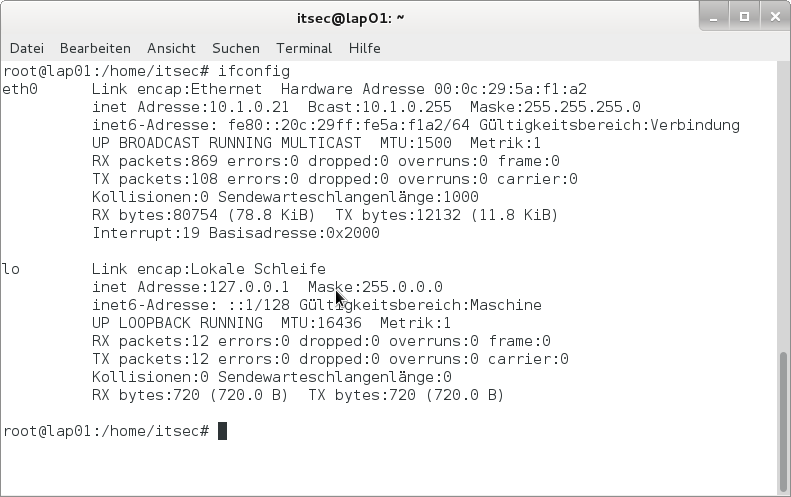
\includegraphics[width=0.7\textwidth]{figures/vpn_ifconfig_lap01.png}
  \caption{Netzwerk-Interfacekonfiguration mit nicht aktiver VPN}
  \label{vpn:screenshot_ifconfig1}
\end{figure}

\begin{figure}[h!]
  \centering
    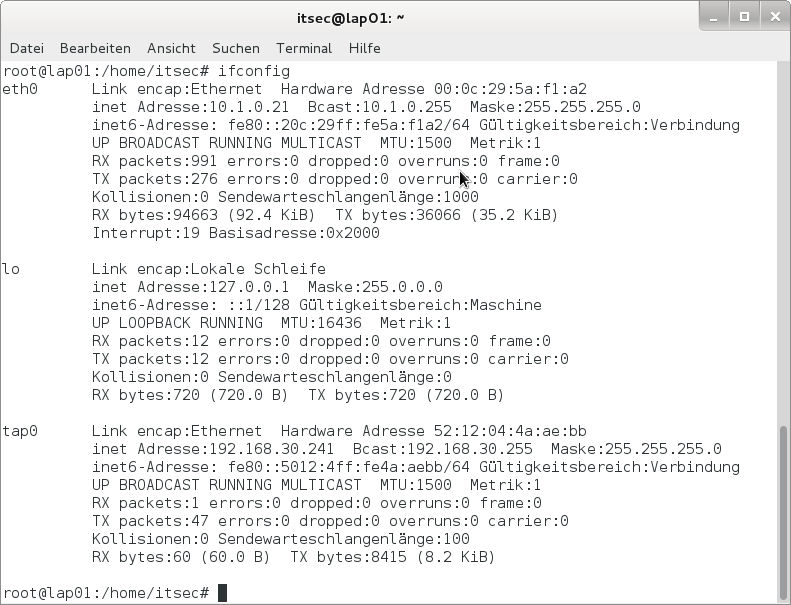
\includegraphics[width=0.7\textwidth]{figures/vpn_ifconfig_lap01_vpn.png}
  \caption{Netzwerk-Interfacekonfiguration mit aktiver VPN}
  \label{vpn:screenshot_ifconfig2}
\end{figure}


Abbildung \ref{vpn:screenshot_ifconfig1} zeigt die Netzwerkschnittstellenkonfiguration ohne aktive VPN-Verbindung, wobei zu erkennen ist, dass nur die beiden Schnittstellen \texttt{eth0} und \texttt{lo} vorhanden sind. Nach dem Start der VPN-Verbindung kommt zusätzlich, wie bereits beschrieben, die \texttt{tap0} Schnittstelle hinzu (siehe Abb. \ref{vpn:screenshot_ifconfig2}), welche die Verbindung zum OpenVPN-Server herstellt. Nach dem Beenden der Verbindung wird sie wieder entfernt.